\documentclass{report}
\usepackage{graphicx}
\usepackage{geometry}
\usepackage{float}
\usepackage{caption}
\usepackage[italian]{babel}

\begin{document}
\captionsetup[table]{name=Figura}

\newgeometry{margin=1in}
\begin{titlepage}


  \noindent
  \begin{minipage}[t]{0.19\textwidth}
    \vspace{-4mm}{
\includegraphics[scale=1.15]{img/logo_unimib.pdf}}
  \end{minipage}
  \begin{minipage}[t]{0.81\textwidth}
    {
      {\textsc{Università degli Studi di Milano - Bicocca}}\\
      \textbf{Scuola di Scienze}\\
      \textbf{Dipartimento di Informatica, Sistemistica e Comunicazione}\\
      \textbf{Corso di laurea in Informatica}\\
      \par
    }
  \end{minipage}

  \vspace{40mm}

  \begin{center}
    {\LARGE{
        \textbf{Recurrent SASC}}}
  \end{center}

  \vspace{50mm}

  \noindent
  {\large \textbf{Relatore:} \textit{Prof. Gianluca Della Vedova} }

  \noindent
  {\large \textbf{Correlatore:} \textit{Dott. Simone Ciccolella}}

  \vspace{15mm}

  \begin{flushright}
    \textbf{\large Relazione della prova finale di:}
    \large{\textit{Stefano Giacomini}}\\
    \large{\textit{Matricola 829854}}
  \end{flushright}

  \vspace{40mm}
  \begin{center}
    {\large{\bf Anno Accademico 2020-2021}}
  \end{center}

  \restoregeometry

\end{titlepage}
\restoregeometry

{\pagestyle{plain}
  \tableofcontents
  \cleardoublepage}

\chapter{Introduzione}

\section{Problemi di ricorstruzione di alberi filogenetici}
  Prima di cominciare a parlare del recurrent SASC vero e proprio è bene fare una breve introduzione dei concetti che verranno utilizzati.\\
  Un albero filogenetico è un grafico che mostra visivamente la collocazione temporale della separazione fra le linee evolutive che a partire da una data specie ha portato alla formazione di due o più specie diverse attraverso una serie di biforcazioni. Con filogenesi basata su caratteri, dove con carattere si intende una qualunque caratteristica che si può osservare, si intende quella filogenesi che sfrutta alcuni caratteri specifici, un esempio può essere la presenza o meno della colonna vertebrale, per rappresentare la storia evolutiva di alcune specie.
  Utilizzando questo concetto e applicandolo, invece che alla separazione di due linee evolutive dovuta ad una serie di mutazioni, all'acquisizione di una cellula di una determinata mutazione, si può rappresentare l'evoluzione di cellule tumorali.\\
  Come menzionato precedentemente la ricostruzione della progressione evolutiva di cellule tumorali può essere modellato con la costruzione di una filogenesi incompleta basata sui caratteri, dove ogni carattere rappresenta una mutazione.
  Consideriamo quindi come input una matrice  ${I}_{ij}$ di dimensioni $n$ x $m$, con $n$ numero delle cellule e $m$ numero delle mutazioni, e dove ${I}_{ij} = 0$ indica che la sequenza $i$ non ha la mutazione $j$, ${I}_{ij} = 1$ indica la presenza della mutazione $j$ nella sequenza $i$ e ? indica che non ci sono abbastanza informazioni sulla presenza/assenza di una mutazione $j$ nella sequenza $i$. Questa incertezza sulla presenza di una mutazione deriva da una insufficiente precisione nel sequenziamento del DNA/RNA.\\
  Oltre a questo ci sono altri problemi derivanti dal sequenziamento, infatti i valori della matrice di input possono anche contenere falsi positivi e falsi negativi, mentre la probabilità di falso positivo è in genere abbastanza bassa, la probabilità di falso negativo può essere alta e variare da una mutazioni all'altra.
  Quindi, detta $E_{ij}$ la matrice $n$ x $m$ di output finale, ovvero la matrice binaria senza errori o rumore prodotto dall'algoritmo, allora ${\alpha}_{j}$ indica la probabilità di falso negativo della mutazione $j$, mentre invece $\beta$ indica la probabilità di falso positivo.\\
  Di conseguenza, per ogni valore di ${E}_{ij}$, valgono le seguenti:
  \[
    P(I_{ij} = 0|{E}_{ij} = 0) = 1 - \beta P(I_{ij} = 0|E_{ij} = 1) = \alpha_{j}
  \]
  \[
    P(I_{ij} = 1|E_{ij} = 0) = \beta P(I_{ij} = 1|E_{ij} = 1) = 1 - \alpha_{j}
  \]
  Puntiamo quindi a trovare una matrice che massimizzi la likelihood della matrice osservata $I$ sotto la probabilità di falso negativo/positivo e i valori mancanti.
  Il nostro lavoro contiene in più la perdita di mutazioni e la possibilità di avere più ricorrenze della stessa mutazione, andiamo quindi a definire $P(L(j))={\gamma}_{j}$ come la probabilità di perdità della mutazione $j$ e il set di variabili ${c}_{j}$ per $j=1,...,m$ che denota il numero totale di perdite per la mutazione $j$ nell'albero.
  Definiamo poi $P(D(j))={\delta}_{j}$ come la probabilità di creare una copia della mutazione $j$ e il set di variabili ${f}_{j}$ per $j=1,...,m$ che denota il numero totale di copie per la mutazione $j$ presenti nell'albero.\\
  Un albero filogenetico $T$ di un set $C$ di $m$ mutazioni e $n$ cellule (affette da queste mutazioni) è definito come un albero con radice i cui nodi interni sono etichettati con le mutazioni di $C$, mentre le foglie sono etichettate dalle cellule.\;\'E importante far notare come l'etichettamento dei nodi deve rispettare alcune restrizioni a seconda del modello evolutivo che stiamo considerando. Per esempio, in una filogenesi perfetta, non possono esistere due nodi con la stessa etichetta.
  Questa è un'alternativa della classica filogenesi basata su caratteri, dove l'albero $T$ è definito come un set di caratteri e dove le foglie non hanno nessuna etichetta e rappresentano specie differenti.\\
  Lo \emph{stato} di un nodo $x$ è definito come il set di mutazioni acquisite ma non perse nel percorso dalla radice a $x$. Lo stato di ogni foglia $l$ di $T$ è rappresentato da un vettore binario di lunghezza $m$, chiamato profilo del genotipo, che denotiamo come $D(T, l)$, dove $D{(T, l)}_{j}=1$ se e solo se la foglia $l$ ha la mutazione $j$ e 0 altrimenti.\\
  Diciamo che l'albero $T$ \emph{codifica} una matrice $E$ se esiste una mappatura $\sigma$ delle righe (cellule) di $E$ nelle foglie di $T$ tale che $E_{i}=D(T, \sigma)_{i}$ per ogni riga $i$ di $E$, dove ${\sigma}_{i}$ denota l'immagine di una riga $i$ attraverso la mappatura $\sigma$.
  Detto in maniera meno formale, ${\sigma}_{i}$ è il nodo dell'albero filogenetico corrispondente al nodo a cui la cellula $i$ è attaccato. Notare come la matrice $E$ è completamente caratterizzata dalla coppia $D(T, \sigma)$. Dunque il nostro problema può essere espresso come trovare l'albero $T$ che massimizzi la seguente funzione obiettivo:
  \[
    \max{\sum_{j}^{m}[-c_{j}\log(1-P(L(j)))-f_{j}\log(1-P(D(j)))+\sum_{i}^{n}\log(P(I_{ij}|D(T, \sigma_{i})_{j}))]}
  \]
  Facciamo inoltre notare come i valori assegnati alle entrate sconosciute della matrice di input non contano nel calcolo della funzione obiettivo, ovvero $P(I_{ij}=\ ?|E_{ij}=1)=P(I_{ij}=\ ?|E_{ij}=0)$. Per semplificare il calcolo della likelihood supponiamo che $P(I_{ij}=\ ?|E_{ij}=1)=P(I_{ij}=\ ?|E_{ij}=0)=1$.
  In più $\sigma$ può essere computato direttamente da $T$, lasciando quindi $T$ come unica variabile da ottimizzare.

\section{Dollo-k e Camil-Socal-k}
  La regola di parsinomia di Dollo assume che in filogenesi ogni singola mutazione è introdotta una sola volta nella storia evolutiva, ma che invece perdite della stessa possono occorrere un numero infinito di volte. Una restrizione del modello di Dollo è ottenibile limitando il numero di perdide per ogni mutazione. Chiamiamo quindi Dollo-$k$ il modello evolutivo in cui ogni mutazione può essere acquisita solo una volta e persa al massimo $k$ volte. I casi speciali Dollo-0 e Dollo-1 corrispondono rispettivamente ai modelli di perfetta e persistente filogenesi.\\
  Invece il modello di Camil-Socal permette molteplici occorrenze della stessa mutazione ma nessuna perdita. Definiamo quindi Camil-Socal-$k$ il modello evolutivo in cui una mutazione può avere al più $k$ ripetizioni e non può mai essere persa. Il caso speciale Camil-Socal-0 corrisponde al modello di filogenesi perfetta.\\
  Il modello utilizzato in questo lavoro è il Car-($k, r$), un modello che va ad unire i modelli introdotti precedentemente e che quindi ammette al massimo $k$ perdite (o backmutation) e $r$ ripetizioni (o recurrent mutation). Dove i modelli di filogenesi perfetta e filogenesi persistente si ottengono rispettivamente con i casi Car-(0, 0) e Car(1, 0). Il problema di ricorstruzione della filogenesi su un modello Car-($k, r$) è NP-completo per ogni $k$ $>$ 1 e $r$ $>$ 0.\\
  Visto che il modello Carl(l, r) utilizza sia backmutation che recurrent mutation introduciamo due nuovi tipi di nodi nell'albero filogenetico, per esprimere le perdite e le ripetizioni delle mutazioni. Per ogni mutazione $p$ creiamo $k$ nuove mutazioni ${p^-}_{l}$ per ogni $l\in\{i, ..., k\}$, rappresentanti le possibili perdite della mutazione $p$, in più creiamo $r$ nuove mutazioni ${p}_{j}$ per ogni $j\in\{i, ..., r\}$ reppresentanto le possibili copie della mutazione $p$.
  In più imponiamo delle nuove regole: che ogni nodo etichettato da una perdita di una mutazione $p^-$ debba essere discendente di un nodo etichettato dall'acquisizione di una mutazione $p$, e che ogni nodo etichettato da $p$ non possa essere discendente di un'altro nodo etichettato con $p$, a meno che questo non sia prima stato perso con un nodo $p^-$.\\
  \'E importante sottolineare come, a differenza del modello a filogenesi perfetta, con l'introduzione di perdite e ricorrenze potremmo avere più alberi che sono soluzione del problema.

  \subsection{Modello utilizzato}
  Nel modello utilizzato sono state in più aggiunte le seguenti restrizioni: il numero massimo di perdite nell'intero albero è al massimo $d$ e il numero di copie è al massimo $z$.\\
  Questo fa si che la variabile $c$ sia soggetta a (i) ${c}_{j}\geq k \ \forall j$ e (ii) $\sum_{j}^m {c}_{j} \geq d$ e che in maniera analoga la variabile $f$ sia soggetta a (i) ${f}_{j}\geq r \ \forall j$ e (ii) $\sum_{j}^m {f}_{j} \geq z$.
  \'E inoltre importante notare come con un numero di mutazioni $m$ non piccolo, settare la variabile $d$ con un valore abbastanza piccolo, per esempio 5, equivale a settare $k\leq 1$, rendendo quindi il valore di k irrilevante; un discorso analogo può essere fatto per quanto riguarda $r$ e $z$.

  \begin{table}[H]
    \begin{minipage}{0.45\textwidth}
    \centering
    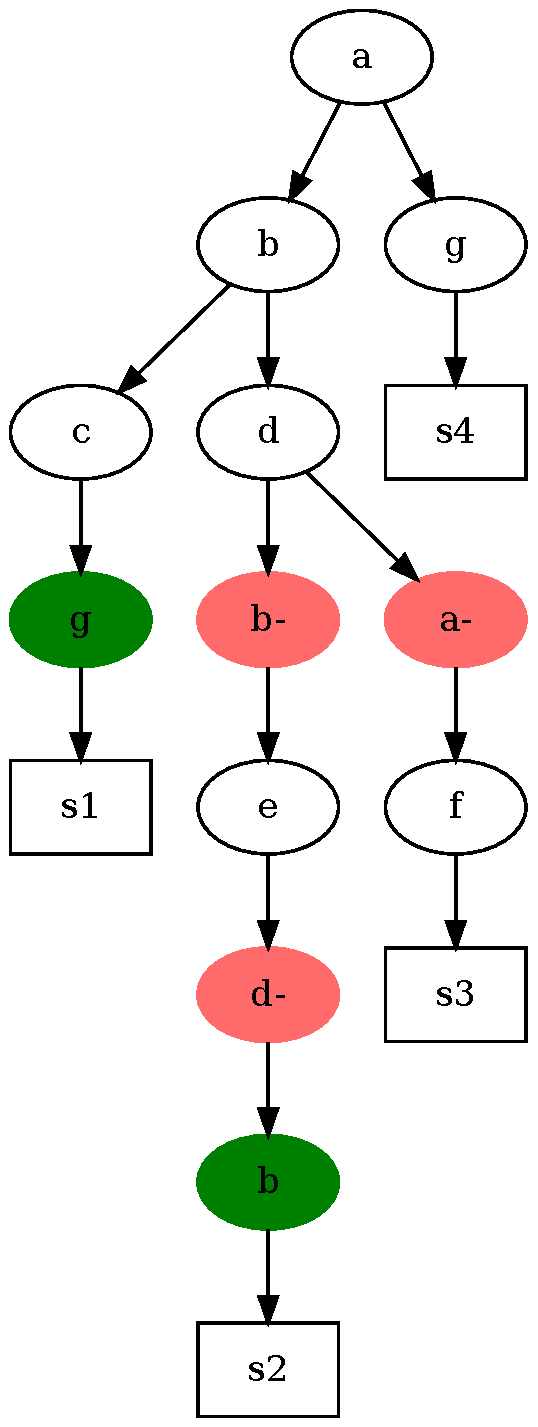
\includegraphics[scale = 0.33]{img/tree.pdf}
    \end{minipage}
    ~\hfill~
    \begin{minipage}{0.5\textwidth}
    \centering
      \begin{tabular}{|l|l|l|l|l|l|l|l|}
        \hline
         & a & b & c & d & e & f & g\\
        \hline
        $s_{1}$ & 1 & 1 & 1 & 0 & 0 & 0 & 1\\
        \hline
        $s_{2}$ & 1 & 1 & 0 & 0 & 1 & 0 & 0\\
        \hline
        $s_{3}$ & 0 & 1 & 0 & 1 & 0 & 1 & 0\\
        \hline
        $s_{4}$ & 1 & 0 & 0 & 0 & 0 & 0 & 1\\
        \hline
      \end{tabular}
    \end{minipage}
    \caption{Esempio di una matrice $E$ (n=4, m=7), a destra, che esprime le cellule $\{ s_{1},...,s_{4}\}$ affette dal set $C = \{ a,...,g\}$ di mutazioni. L'albero $T$, a sinistra, è un albero di filogenesi di cellule tumorali raffigurante la matrice $E$,
    nel quale i nodi rappresentanti le backmutation sono colorati di rosso e i quelli rappresentanti le recurrent mutation sono colorati di verde. \'E importante far notare che la matrice non permette una filogenesi perfetta e che $T$ è una filogenesi Car(1, 1)}
    \label{fig:fig1}
  \end{table}

\section{Simulated Annealing}
  Il fatto che (i) e (ii), e il fatto che vogliamo cercare l'albero che massimizzi la likelihood, rendono il problema di riscostruzione della filogenesi computazionalmente NP-hard sotto il modello Car($k$, $r$) per ogni $k$ o $r > 0$. Per questo motivo si è deciso di utlizzare il metodo del Simulated Annealing (SA) per cercare l'albero che massimizzi la likelihood di una determinata matrice di input, soddisfacendo il modello Car($k$, $r$), dove $k$ e $r$ sono dati come input.
  SA è una metaeuristica che sfrutta un metodo di ricerca randomico che esplora la regione delle soluzioni ammissibili alla ricerca dell'ottimo, esattamente come tutte le altre metaeuristiche non c'è certezza che SA trovi la soluzione ottima della funzione obiettivo in un numero finito di step.\\
  SA è però in grado, rispetto ad altri metodi deterministici, di evitare di rimanere bloccato in ottimi locali in quanto può accettare anche step non migliorativi; nello specifico sia data $X_{c}$, soluzione ammissibile, e $Z_{c}$, valore della funzione obiettivo nel punto $X_{c}$, calcolo $X_{n}$, punto nell'intorno di $X_{c}$ calcolato da una mossa randomica, se $Z_{n}$, valore della funzione obiettivo in $X_{n}$, è migliore di $Z_{c}$, allora $X_{n}$ diventa il nuovo $X_{c}$, altrimenti ho comunque una probabilità che questo avvenga ed è pari a: $e^{\frac{Z_{n}-Z_{c}}{T}}$.
  Con $T$ che è una variabile chiamata \emph{temperatura} scelta inizialmente e che continua a diminuire nel tempo dopo un certo numero di mosse non migliorative.\\
  Come si può intuire dalla formula, una temperatura alta indica una più alta probabilità di accettare mosse molto peggiorative, favorendo l'\emph{exploration}, ovvero la ricerca all'interno della funzione per evitare di rimanere incastrati in ottimi locali, invece man mano che la temperatura diminuisce anche la probabilità di accettare mosse molto peggiorative, favorendo quindi l'\emph{exploitation}, ovvero la ricerca dell'ottimo nell'intorno in cui mi trovo, con $T\approx 0$ non accetto più soluzioni peggiorative. Il criterio di arresto dell'algoritmo in genere è l'aver fatto un certo numero di iterazioni con una $T$ minima, scelta inizialmente.

\chapter{World}

\section{End}
  End.



\end{document}
